\documentclass[conference,a4paper]{IEEEtran}
\IEEEoverridecommandlockouts
\usepackage{cite}
\usepackage{amsmath,amssymb,amsfonts}
\usepackage{algorithmic}
\usepackage{graphicx}
\usepackage{textcomp}
\usepackage{xcolor}
\usepackage{booktabs}
\usepackage{algorithm}
\usepackage{float} 

\def\BibTeX{{\rm B\kern-.05em{\sc i\kern-.025em b}\kern-.08em
    T\kern-.1667em\lower.7ex\hbox{E}\kern-.125emX}}

\begin{document}

\title{Optimizing Household Waste Segregation Policy in the Municipality of Bacolod: An Agent-Based Modeling and Heuristic-Guided Deep Reinforcement Learning Approach}

\author{
\IEEEauthorblockN{1\textsuperscript{st} Jemar John J. Lumingkit}
\IEEEauthorblockA{\textit{Department of Computer Science} \\
\textit{Mindanao State University -}\\
\textit{Iligan Institute of Technology}\\
Iligan City, Philippines \\
jemarjohn.lumingkit@g.msuiit.edu.ph}
\and
\IEEEauthorblockN{2\textsuperscript{nd} Hussam M. Bansao}
\IEEEauthorblockA{\textit{Department of Computer Science} \\
\textit{Mindanao State University -}\\
\textit{Iligan Institute of Technology}\\
Iligan City, Philippines \\
hussam.bansao@g.msuiit.edu.ph}
\and
\IEEEauthorblockN{3\textsuperscript{rd} Dante D. Dinawanao}
\IEEEauthorblockA{\textit{Department of Computer Science} \\
\textit{Mindanao State University -}\\
\textit{Iligan Institute of Technology}\\
Iligan City, Philippines \\
dante.dinawanao@g.msuiit.edu.ph}
}

\maketitle

\begin{abstract}
The implementation of the Ecological Solid Waste Management Act (RA 9003) remains a critical challenge for Local Government Units (LGUs) in the Philippines, primarily hindered by chronic budget constraints and the complexity of predicting behavioral dynamics. This study presents a novel computational governance framework combining Agent-Based Modeling (ABM) with Deep Reinforcement Learning (DRL) to optimize public policy allocation in the Municipality of Bacolod. We formulated the municipal ecosystem as a Markov Decision Process (MDP), where a multi-level ABM simulates heterogeneous household agents reacting to municipal interventions governed by a dynamically weighted Theory of Planned Behavior (TPB). A centralized ``Mayor Agent,'' powered by a Heuristic-guided DRL (HuDRL) architecture, is trained to maximize municipality-wide segregation compliance under strict fiscal limits. Global Sensitivity Analysis using the Sobol method reveals that the ``Cost of Effort'' accounts for 78\% of non-compliance variance, mathematically validating the necessity of logistical interventions over pure awareness campaigns. Consequently, simulations demonstrate that the HuDRL agent out-performs traditional equitable distribution heuristics by achieving 90.45\% global compliance. The AI autonomously discovered an aggressive ``Sequential Saturation'' strategy, concentrating capital on singular bottlenecks to induce permanent socio-behavioral tipping points rather than diluting resources municipality-wide.
\end{abstract}

\begin{IEEEkeywords}
Agent-Based Modeling, Deep Reinforcement Learning, Smart Governance, Markov Decision Process, Theory of Planned Behavior
\end{IEEEkeywords}

\section{Introduction}

\subsection{Background}
The national framework for solid waste management in the Philippines is anchored by the Ecological Solid Waste Management Act (R.A. 9003), mandating rigorous source segregation and decentralized, barangay-level processing \cite{ra9003, yazawa2025}. However, practical implementation remains suboptimal at the local government level. LGUs, particularly resource-constrained municipalities like Bacolod, Lanao del Norte, operate under severe fiscal, logistical, and manpower limitations that cripple enforcement capabilities.

\subsection{Problem Statement}
Traditional local governance attempts to manage these constraints through static, blanket policies—such as uniform penalty fees or equitable budget distribution across all jurisdictions. These heuristics fail because they do not account for socio-economic heterogeneity or the adaptive nature of human behavior \cite{tian2024, nishimura2022}. When LGUs apply uniform policies to a non-uniform populace, financial resources are inevitably diluted below the critical threshold required to alter established social norms, resulting in systemic non-compliance.

\subsection{Objectives}
Addressing these persistent behavioral challenges requires a shift toward predictive, smart governance. This study proposes a coupled Agent-Based Modeling (ABM) and Heuristic-Guided Deep Reinforcement Learning (HuDRL) framework tailored for the Municipality of Bacolod. By transforming psychological behavioral models into a mathematical interface for a DRL algorithm, we elevate the LGU from a reactive administrator to a strategic learner, providing a risk-free, cost-effective computational tool to maximize long-term household compliance.

\section{Related Work}

\subsection{Behavioral Tipping Points}
The core mechanics of behavioral adoption in complex networks are well-documented. Centola et al. \cite{centola2018} established that transitioning a population's behavior does not require independent adoption by the absolute majority; instead, overwhelming a critical mass threshold (often 25\% to 40\%) triggers a rapid cascade of adoption across the network. This ``Graduation Effect'' implies that reaching a localized tipping point locks in the behavior through cultural inertia \cite{andre2021}, allowing an LGU to subsequently withdraw active funding without the community relapsing into non-compliance.

\subsection{Policy Interventions}
To enforce waste segregation, LGUs typically employ a mix of educational campaigns and penalties. However, environmental sociology highlights a profound ``Intention-Action Gap'' \cite{paigalan2025}. While education effectively improves intrinsic attitudes, it exhibits diminishing returns when structural friction is high. Extrinsic motivators, such as hybrid reward-penalty schemes, are significantly more effective in developing nations because they directly alter the financial cost-benefit analysis of the residents \cite{zhao2022, moeini2023}.

\subsection{ABM and DRL in Governance Simulations}
Agent-Based Modeling functions as a ``virtual laboratory,'' uniquely equipped to capture population heterogeneity and economic disparities that macro-level System Dynamics models miss \cite{taraghi2025}. While ABM provides the environment, Deep Reinforcement Learning (DRL) is essential for autonomously discovering optimal policies within high-dimensional state spaces. Currently, DRL is extensively utilized for physical waste sorting and collection routing \cite{zheng2022b, udayakumar2023}. However, its application in optimizing governance resources to actively influence human behavior remains critically under-explored. 

\section{Methodology}

\subsection{Research Architecture and Simulation Bounds}
This study integrated ABM with DRL optimization in a three-phase design: parameterization, DRL integration, and scenario simulation. The environment is geographically bounded to the seven coastal and urban barangays of Bacolod currently served by the municipal collection system. The simulation projects over a multi-year horizon using quarterly time steps. The central constraint is a strict annual municipal budget of \textpeso 1,500,000. This hard fiscal boundary creates a realistic ``Personnel Trap'' \cite{nishimura2022}. Because enforcement agents require a mandatory daily minimum wage, over-investing in punitive measures mathematically crowds out the remaining policy levers. Since the DRL agent's continuous Action Space ($\mathcal{A}$) is strictly bounded by a Softmax normalization layer, any aggressive deployment of personnel creates a zero-sum collapse in available funding for community incentives or awareness campaigns. The complete simulation architecture outlining this dual-clock polycentric framework is illustrated in Figure \ref{fig:simul_diagram}.

\begin{figure}[H] 
\centering
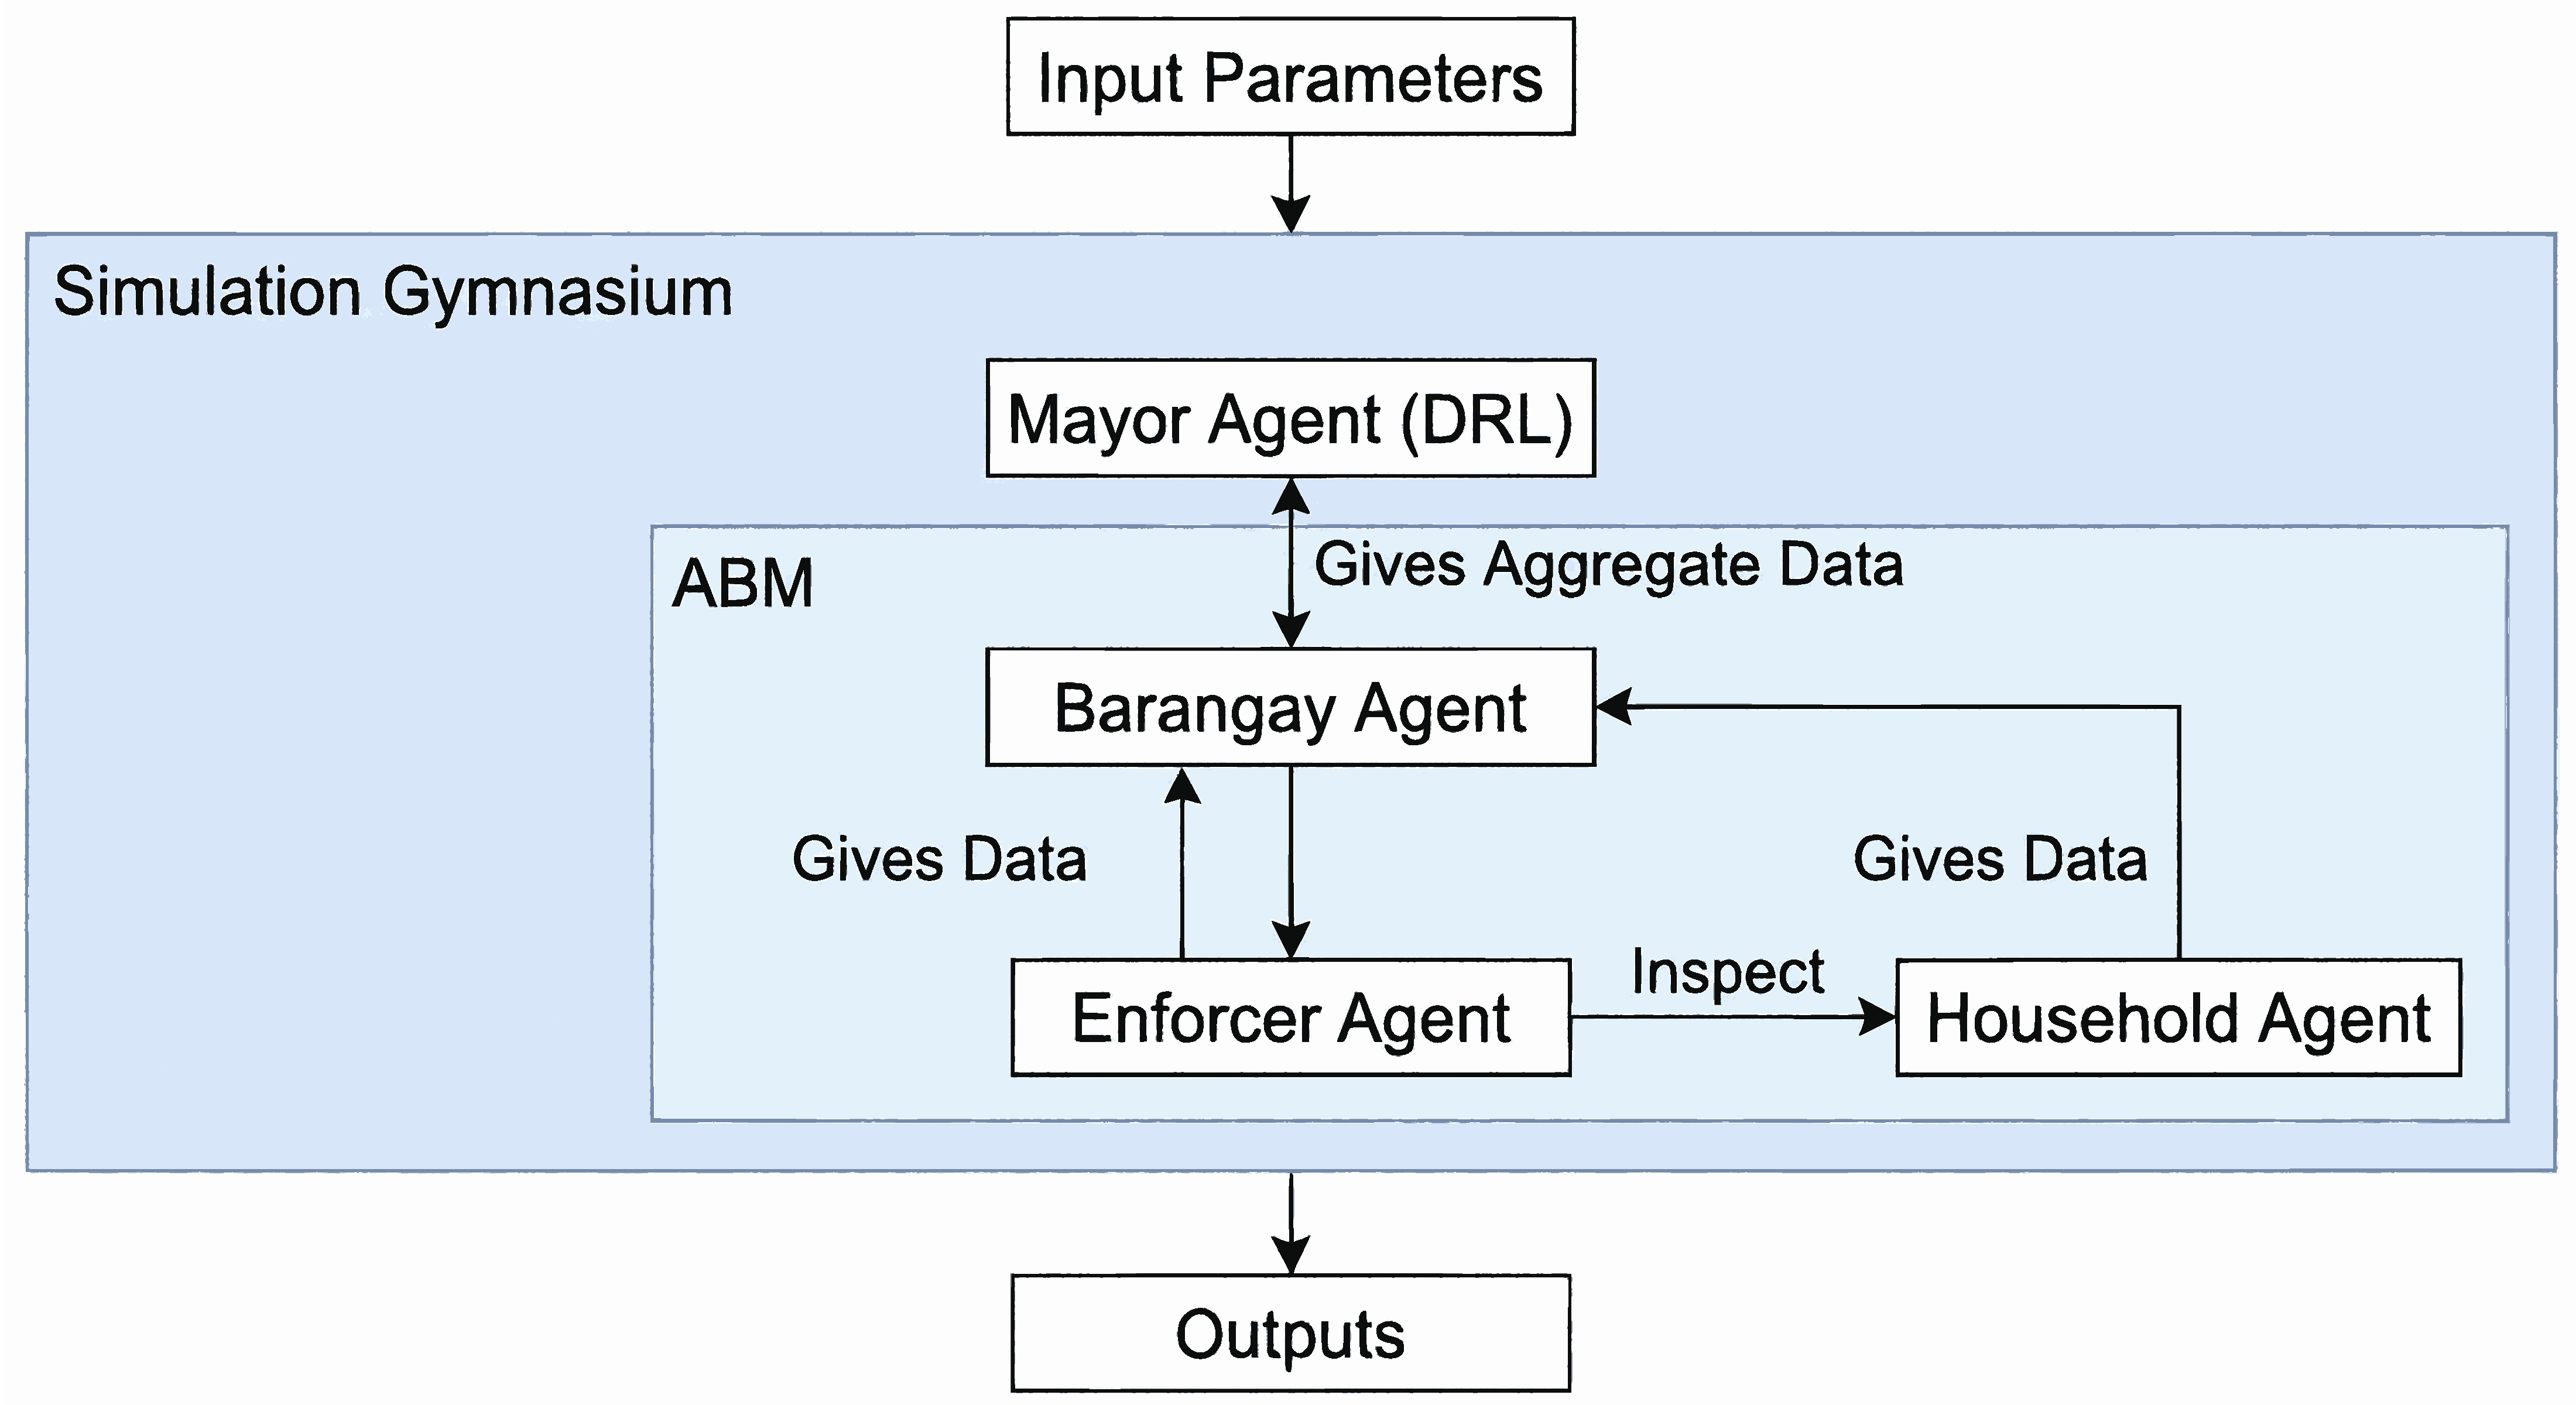
\includegraphics[width=0.85\columnwidth]{images/simul_gym.png}
\caption{Simulation Architecture Diagram}
\label{fig:simul_diagram}
\vspace{-0.3cm}
\end{figure}

\subsection{Markov Decision Process (MDP) Formulation}
To facilitate the integration of the Deep Reinforcement Learning algorithm, the entire multi-agent ecosystem is mathematically formulated as an episodic Markov Decision Process (MDP) \cite{zheng2022b}, defined by the tuple $\langle \mathcal{S}, \mathcal{A}, \mathcal{P}, \mathcal{R}, \gamma \rangle$:
\begin{itemize}
    \item \textbf{State Space ($\mathcal{S}$):} A continuous vector representing the aggregated quarterly compliance rate of each barangay, the remaining LGU budget, and the current simulation time step.
    \item \textbf{Action Space ($\mathcal{A}$):} The continuous allocation percentages of the quarterly budget across three levers (Enforcement, Incentives, Education) mapped to specific barangays.
    \item \textbf{Transition Dynamics ($\mathcal{P}$):} The non-deterministic socio-behavioral evolution of the ABM environment in response to $\mathcal{A}$.
\end{itemize}

\subsection{Multi-Level ABM Architecture}

\subsubsection{Household Agents}
Household agents operate as continuous finite state machines executing binary waste segregation choices. To ensure population heterogeneity, behavioral weights are instantiated via stochastic Gaussian sampling $\mathcal{N}(\mu, \sigma^2)$, bounded within $[0.1, 0.6]$. This ensures that systemic compliance emerges organically from individualized, micro-level cost-benefit analyses. Their cognition is governed by a dynamically weighted Theory of Planned Behavior (TPB) utility equation ($U_{seg}$) \cite{taraghi2025}:
\begin{equation}
\begin{split}
U_{seg} = &(w_{A}(t)A) + (w_{SN}(t)SN_{loc}) \\
&+ (w_{PBC}(t)PBC) - C_{Net} + \epsilon
\end{split}
\end{equation}
Where $A$, $SN_{loc}$, and $PBC$ represent Attitude, localized Subjective Norms, and Perceived Behavioral Control, buffered by stochastic human noise ($\epsilon$).

A critical computational feature is the Net Cost ($C_{Net}$) function, which translates abstract psychological friction into a computable scalar:
\begin{equation}
    C_{Net} = C_{Effort} + \gamma (C_{Mon} - I - F \cdot P_{Detect})
\end{equation}
Here, the physical hassle ($C_{Effort}$) is weighed against financial variables: tangible costs ($C_{Mon}$), municipal incentives ($I$), and expected fines ($F \times P_{Detect}$) \cite{zhao2022}. These financial vectors are scaled by $\gamma$, an income-sensitivity multiplier where lower-income agents assign exponentially higher psychological weight to monetary levers.

To accurately model ``Cultural Inertia,'' the agent queries its immediate spatial environment using an $\mathcal{O}(k)$ Moore neighborhood algorithm to calculate $SN_{loc}$. The simulation implements a state-dependent ``Social Norm Shield.'' During the daily decision execution tick, if localized compliance breaches a 70\% tipping point ($SN_{loc} \ge 0.70$), the behavior transitions from a financially calculated decision to an internalized convention \cite{centola2018}. The agent's subjective norm weight mathematically hard-locks ($w_{sn} = 0.90$), heavily resisting negative behavioral decay. Conversely, if $SN_{loc} < 0.40$, the shield fails, forcing the agent to rely strictly on external enforcement. Ultimately, if the evaluated overall benefits ($U_{seg}$) outweigh the Net Effort ($C_{Net}$), the agent successfully segregates its waste, subject to a 1\% stochastic failure rate simulating natural human error. The synthesis of this process is detailed in Algorithm \ref{alg:household_decision_english}.

\begin{algorithm}[H] 
\caption{The Household's Daily Decision Process}
\label{alg:household_decision_english}
\begin{algorithmic}[1]
\STATE \textbf{Input:} Income Sensitivity ($\gamma$), Attitude ($A$), Peer Pressure ($SN_{loc}$), Base Effort ($C_{Effort}$)
\STATE \textbf{Step 1: Evaluate Peer Pressure \& The Habit Shield}
\STATE Calculate local compliance ($SN_{loc}$) by checking neighbors.
\IF{$SN_{loc} \ge 0.70$}
    \STATE \textit{Apply Habit Shield:} Lock peer pressure weight.
\ELSIF{$SN_{loc} < 0.40$}
    \STATE \textit{Shield Fails:} Rely strictly on external enforcement.
\ENDIF
\STATE \textbf{Step 2: Update Motivation \& Calculate Net Effort}
\STATE Apply natural attitude decay, buffered by IEC boosts.
\STATE Calculate Net Effort ($C_{Net}$) using physical hassle, fines, and rewards (scaled by $\gamma$).
\STATE Calculate total Utility ($U_{seg}$) and add random error.
\STATE \textbf{Step 3: Execute the Final Choice}
\IF{Overall benefits ($U_{seg}$) $>$ Net Effort}
    \STATE Roll a 1\% chance of accidental failure.
    \IF{Passed} \STATE \textbf{Action:} Successfully segregate waste. \ENDIF
\ELSE
    \STATE \textbf{Action:} Do not segregate.
\ENDIF
\end{algorithmic}
\end{algorithm}
\vspace{-0.4cm}

\subsubsection{Enforcement Agents (Operational Arm)}
Acting as the punitive actuators of the simulation, enforcement agents physically manifest the fine ($F$) and perceived risk ($P_{Detect}$) variables. The architecture bifurcates into two operational profiles: \textit{Micro-Enforcers} (Barangay Tanods) simulate persistent local watchmen but execute a 90\% stochastic distraction filter, frequently skipping patrols to mimic real-world multitasking. Conversely, \textit{Macro-Enforcers} (LGU Strike Force) are spawned directly by the AI Mayor for dedicated, high-capacity patrols. To prevent memory leaks and simulate logistical realities, these objects are bound by strict 30-day temporal contracts, forcing the DRL agent to continuously justify their budgetary upkeep \cite{yazawa2025}.

To simulate bounded rationality, enforcers lack $\mathcal{O}(1)$ global oversight \cite{tian2024}. Instead, they execute stochastic random-walks and localized $\mathcal{O}(r^2)$ Moore neighborhood spatial queries to detect non-compliant households. The aggregate inspection capacity ($C$) of these deployed agents dynamically generates the macro-level probability of detection:
\begin{equation}
    P_{Detect} = \min\left(1.0, \frac{\sum C_{Quarterly}}{N_{Households}}\right)
\end{equation}
This scalar is continuously broadcasted back to the household agents. This organically generates a fluctuating risk profile strictly constrained by the physical logistics of the simulated LGU.

\subsubsection{Barangay Agents}
Representing the seven demographic zones, these agents serve as localized administrative nodes bridging micro-level behavior and macro-level policy. Computationally, they aggregate household data in $\mathcal{O}(N_b)$ time to calculate the localized compliance rate ($R_{bgy}$). This metric is passed to the centralized MDP to form the state observation space ($\mathcal{S}$) and locally triggers the 70\% Social Norm Shield. Furthermore, each barangay executes a static baseline policy utilizing its localized Internal Revenue Allotment (IRA) \cite{nishimura2022}.

Crucially, to simulate polycentric governance, the agent operates a \textit{cascading incentive protocol}. When compliant households claim financial rewards, the agent draws first from its local IRA funds, and second from the AI Mayor's targeted municipal augmentation budget. If both budget tiers are exhausted, the claim is rejected. This rejection triggers a computational ``Perceived Unfairness'' penalty that severely degrades the household's future intrinsic motivation, simulating a ``victim of success'' dynamic \cite{moeini2023}.

\subsection{Mayor Agent with Heuristic-Guided DRL (HuDRL)}

\subsubsection{Proximal Policy Optimization}
The LGU policymaker (the ``Mayor Agent'') is powered by an Actor-Critic Proximal Policy Optimization (PPO) neural network \cite{zheng2022b}. The Actor network outputs continuous budget allocations strictly bounded by a Softmax normalization layer. As established by the ``Personnel Trap,'' this layer guarantees the \textpeso 1,500,000 fiscal limit is never breached by forcing the multi-dimensional action vector to sum to exactly 100\% of available funds. Concurrently, the Critic network evaluates the expected long-term return, utilizing PPO's clipped surrogate objective to prevent catastrophic policy shifts during training \cite{udayakumar2023}. To ensure computational reproducibility, the neural network architecture comprises two fully connected hidden layers of 64 units each for both the Actor and Critic networks, utilizing Rectified Linear Unit (ReLU) activation functions. The model is trained with a discount factor ($\gamma$) of 0.99, a learning rate of $0.0003$, a rollout buffer of 1024 steps, a batch size of 128, and an entropy coefficient of 0.01.

\subsubsection{Multi-Objective Reward Shaping}
Directing human behavior introduces the ``Sparse Reward Problem,'' where delayed causal effects cause standard AI agents to fail \cite{zheng2022b}. This necessitates a dense feedback architecture capable of evaluating intermediate municipal actions long before the final socio-behavioral tipping points are actually reached. To overcome this, the MDP utilizes a composite reward function ($R_{total}$):
\begin{equation}
\begin{split}
R_{total} = &w_{1}R_{Comp} + w_{2}R_{Sustain} \\
&- w_{3}P_{Backlash} + R_{Shaping}
\end{split}
\end{equation}
This balances environmental compliance ($R_{Comp}$) against fiscal sustainability ($R_{Sustain}$) and public pushback ($P_{Backlash}$). The specific scalar weights were calibrated to balance these competing municipal mandates: $w_1 = 10.0$ (scaling global compliance into a primary baseline reward), $w_2 = 5.0$ (a targeted focus bonus to prioritize funding the weakest barangay), and $w_3 = 2.0$ (a political penalty multiplier applied when public approval drops below 50\%, forcing the agent to balance punitive fines with educational campaigns).

\subsubsection{Targeted Amplification Algorithm}
To prevent the PPO agent from falling into the sub-optimal trap of equitable distribution, $R_{Shaping}$ provides a massive heuristic bonus for concentrating $>40\%$ of the budget on a single failing node. This targeted amplification logic and its integrated safety guardrails are executed continuously via Algorithm \ref{alg:hudrl_triage}.

\begin{algorithm}[H] 
\caption{The Mayor Agent's Triage \& Safety Heuristics}
\label{alg:hudrl_triage}
\begin{algorithmic}[1]
\STATE \textbf{Rule 1: The 70\% Graduation Mechanism}
\FOR{each Barangay}
    \IF{Compliance Rate $\ge 70\%$}
        \STATE Reduce proposed budget allocation by 99\%
    \ENDIF
\ENDFOR
\STATE \textbf{Rule 2: The Phase-Shift Crisis Guardrail}
\STATE Identify the ``Weakest Performer'' (lowest compliance).
\IF{Global Compliance $< 40\%$}
    \STATE Override allocation: Guarantee this weakest barangay receives a minimum of 50\% of the municipal budget.
\ENDIF
\STATE \textbf{Rule 3: Softmax Normalization}
\STATE Apply a Temperature-Scaled Softmax function to ensure outputs sum to exactly 100\% of available funds.
\end{algorithmic}
\end{algorithm}
\vspace{-0.4cm}

\section{Results and Discussion}

\subsection{Data Gathered and Calibration}
Empirical calibration successfully reconciled an ``Act vs. Reality'' discrepancy \cite{yazawa2025}. While interviews with local officials suggested perceived compliance rates of 40-50\%, the Municipal Enviroment and Natural Resources Office (MENRO) audits confirmed actual compliance was 10-15\%. The model utilized Barangay Poblacion (at an audited 2\% compliance) as a high-fidelity anchor to counteract social desirability bias, establishing a valid Status Quo baseline \cite{paigalan2025}. Beyond static calibration, the dynamic behavior of the ABM was structurally validated using qualitative time-series narratives gathered via key informant interviews. By mirroring the historical peaks and rapid decay of past, short-lived LGU interventions (e.g., sporadic ``Eco-bricks for rice'' pop-ups), the model's socio-temporal dynamics and adherence to established ``Stylized Facts'' (such as Centola's tipping points \cite{centola2018}) were structurally validated before DRL training commenced. The synthesized municipal profiles and parameters are summarized in Table \ref{tab:consolidated_data}.

\begin{table}[H] 
    \centering
    \caption{Synthesized Municipal Data and Initialization Parameters}
    \label{tab:consolidated_data}
    \resizebox{0.95\columnwidth}{!}{%
    \begin{tabular}{l r r c c c c c}
        \toprule
        & & & \multicolumn{2}{c}{\textbf{Compliance}} & \multicolumn{3}{c}{\textbf{Behavior Parameters}} \\
        \cmidrule(lr){4-5} \cmidrule(lr){6-8}
        \textbf{Barangay} & \textbf{Pop.} & \textbf{Budget (\textpeso)} & \textbf{Self-Rep.} & \textbf{Calib.} & \textbf{$w_a$} & \textbf{$w_{sn}$} & \textbf{$PBC$} \\
        \midrule
        Poblacion & 1,534 & 200,000 & 2\% & 2\% & 0.25 & 0.15 & 0.20 \\
        Liangan East & 608 & 30,000 & 65\% & 14\% & 0.25 & 0.30 & 0.20 \\
        Ezperanza & 574 & 90,000 & 20\% & 14\% & 0.20 & 0.35 & 0.25 \\
        Binuni & 507 & 126,370 & 95\% & 15\% & 0.40 & 0.45 & 0.35 \\
        Demologan & 463 & 21,000 & 60\% & 11\% & 0.35 & 0.35 & 0.30 \\
        Babalaya & 171 & 15,000 & 100\% & 15\% & 0.35 & 0.50 & 0.35 \\
        Mati & 165 & 80,000 & 70\% & 13\% & 0.30 & 0.40 & 0.25 \\
        \bottomrule
    \end{tabular}%
    }
    \vspace{1ex}
    
    \raggedright
    \footnotesize
    \textit{Note:} Pop. = Household Population; Self-Rep. = Interview-based compliance; Calib. = Calibrated anchor to MENRO audit ($t=0$); Behavior Parameters refer to localized TPB weights.
    \vspace{-0.3cm}
\end{table}

\subsection{Global Sensitivity Analysis on Household Agents}
A Sobol Global Sensitivity Analysis (GSA) \cite{sobol2001} revealed that the ``Cost of Effort'' ($C_{effort}$) is the overwhelmingly dominant driver of behavior, accounting for 78\% of the variance in global compliance ($S_1 \approx 0.78$). This mathematically validates the ``Convenience Hypothesis''—if the physical or financial friction of segregation is high, households will default to non-compliance regardless of environmental beliefs \cite{taraghi2025}. Conversely, the intrinsic Attitude weight ($w_a$) exhibited near-zero sensitivity. This quantifies the ``Value-Action Gap,'' proving that Information Campaigns (IEC) have a strictly limited ceiling of effectiveness when deployed without localized structural support. The distribution of these indices is visualized in Figure \ref{fig:sobol}.

\begin{figure}[H] 
\centering
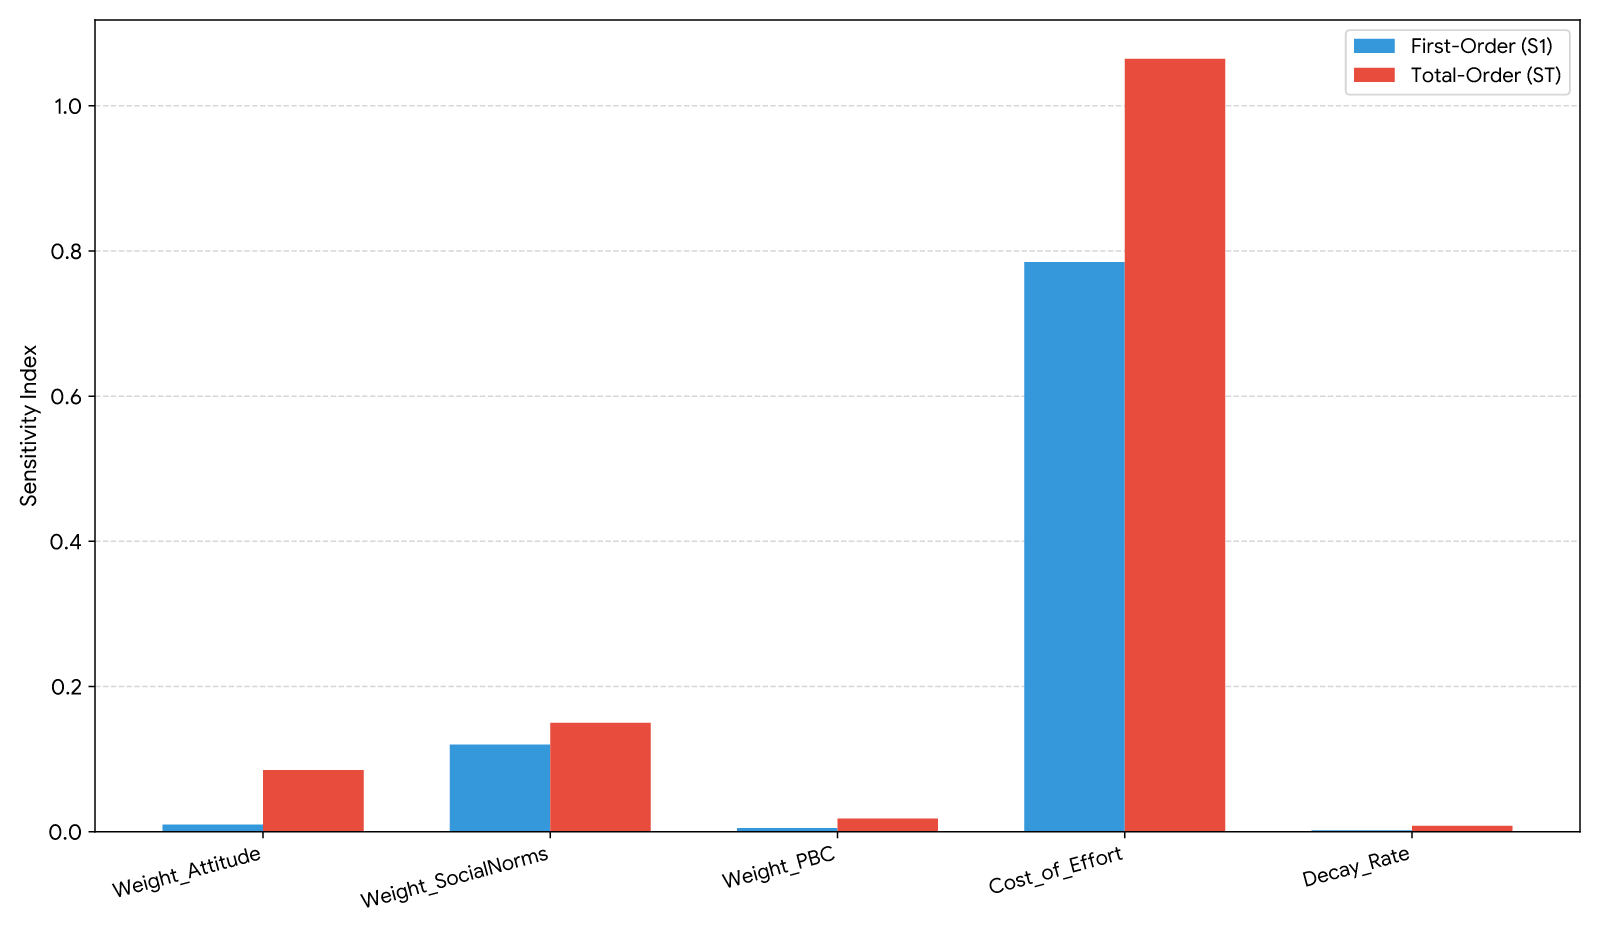
\includegraphics[width=0.85\columnwidth]{images/Sobol.png}
\caption{General Sensitivity Analysis using the Sobol Method}
\label{fig:sobol}
\vspace{-0.3cm}
\end{figure}

\subsection{Comparative Convergence: Heuristic vs. Non-Heuristic PPO}
To evaluate the efficacy of these methodological refinements, the simulation benchmarked the HuDRL architecture against the baseline Non-Heuristic PPO approach over a 12-quarter horizon. Figure \ref{fig:heuristic_vs_non_heuristic} illustrates the Global Compliance Rate trajectories for both models relative to the defined Stability Threshold ($70\%$) and Collapse Zone ($<40\%$).

The \textit{Non-Heuristic Approach} (represented by the dashed grey trajectory) exhibited severe policy stagnation. Throughout the entire 3-year simulation timeline, the global compliance rate remained virtually flat at approximately $20\%$. This performance consistently trapped the municipality within the ``Collapse Zone,'' mathematically proving that without heuristic action-masking or adaptive triage logic, the system failed to concentrate enough capital to incentivize behavioral change due to the sparse reward problem \cite{zheng2022b}.

In stark contrast, the \textit{Heuristic Approach} (solid blue trajectory) demonstrated rapid gradient convergence toward optimal compliance. Starting at a baseline compliance rate of $51.8\%$ in Quarter 1 (under the guided framework), the HuDRL agent successfully navigated the non-convex policy space, breaching the critical $70\%$ Stability Threshold by Quarter 2. By systematically targeting failing sectors via the algorithmic guardrails, the system achieved a near-saturation point by Quarter 6, reaching approximately $98\%$ compliance, and maintained this asymptotic stability through Quarter 12.

\begin{figure}[H] 
    \centering
    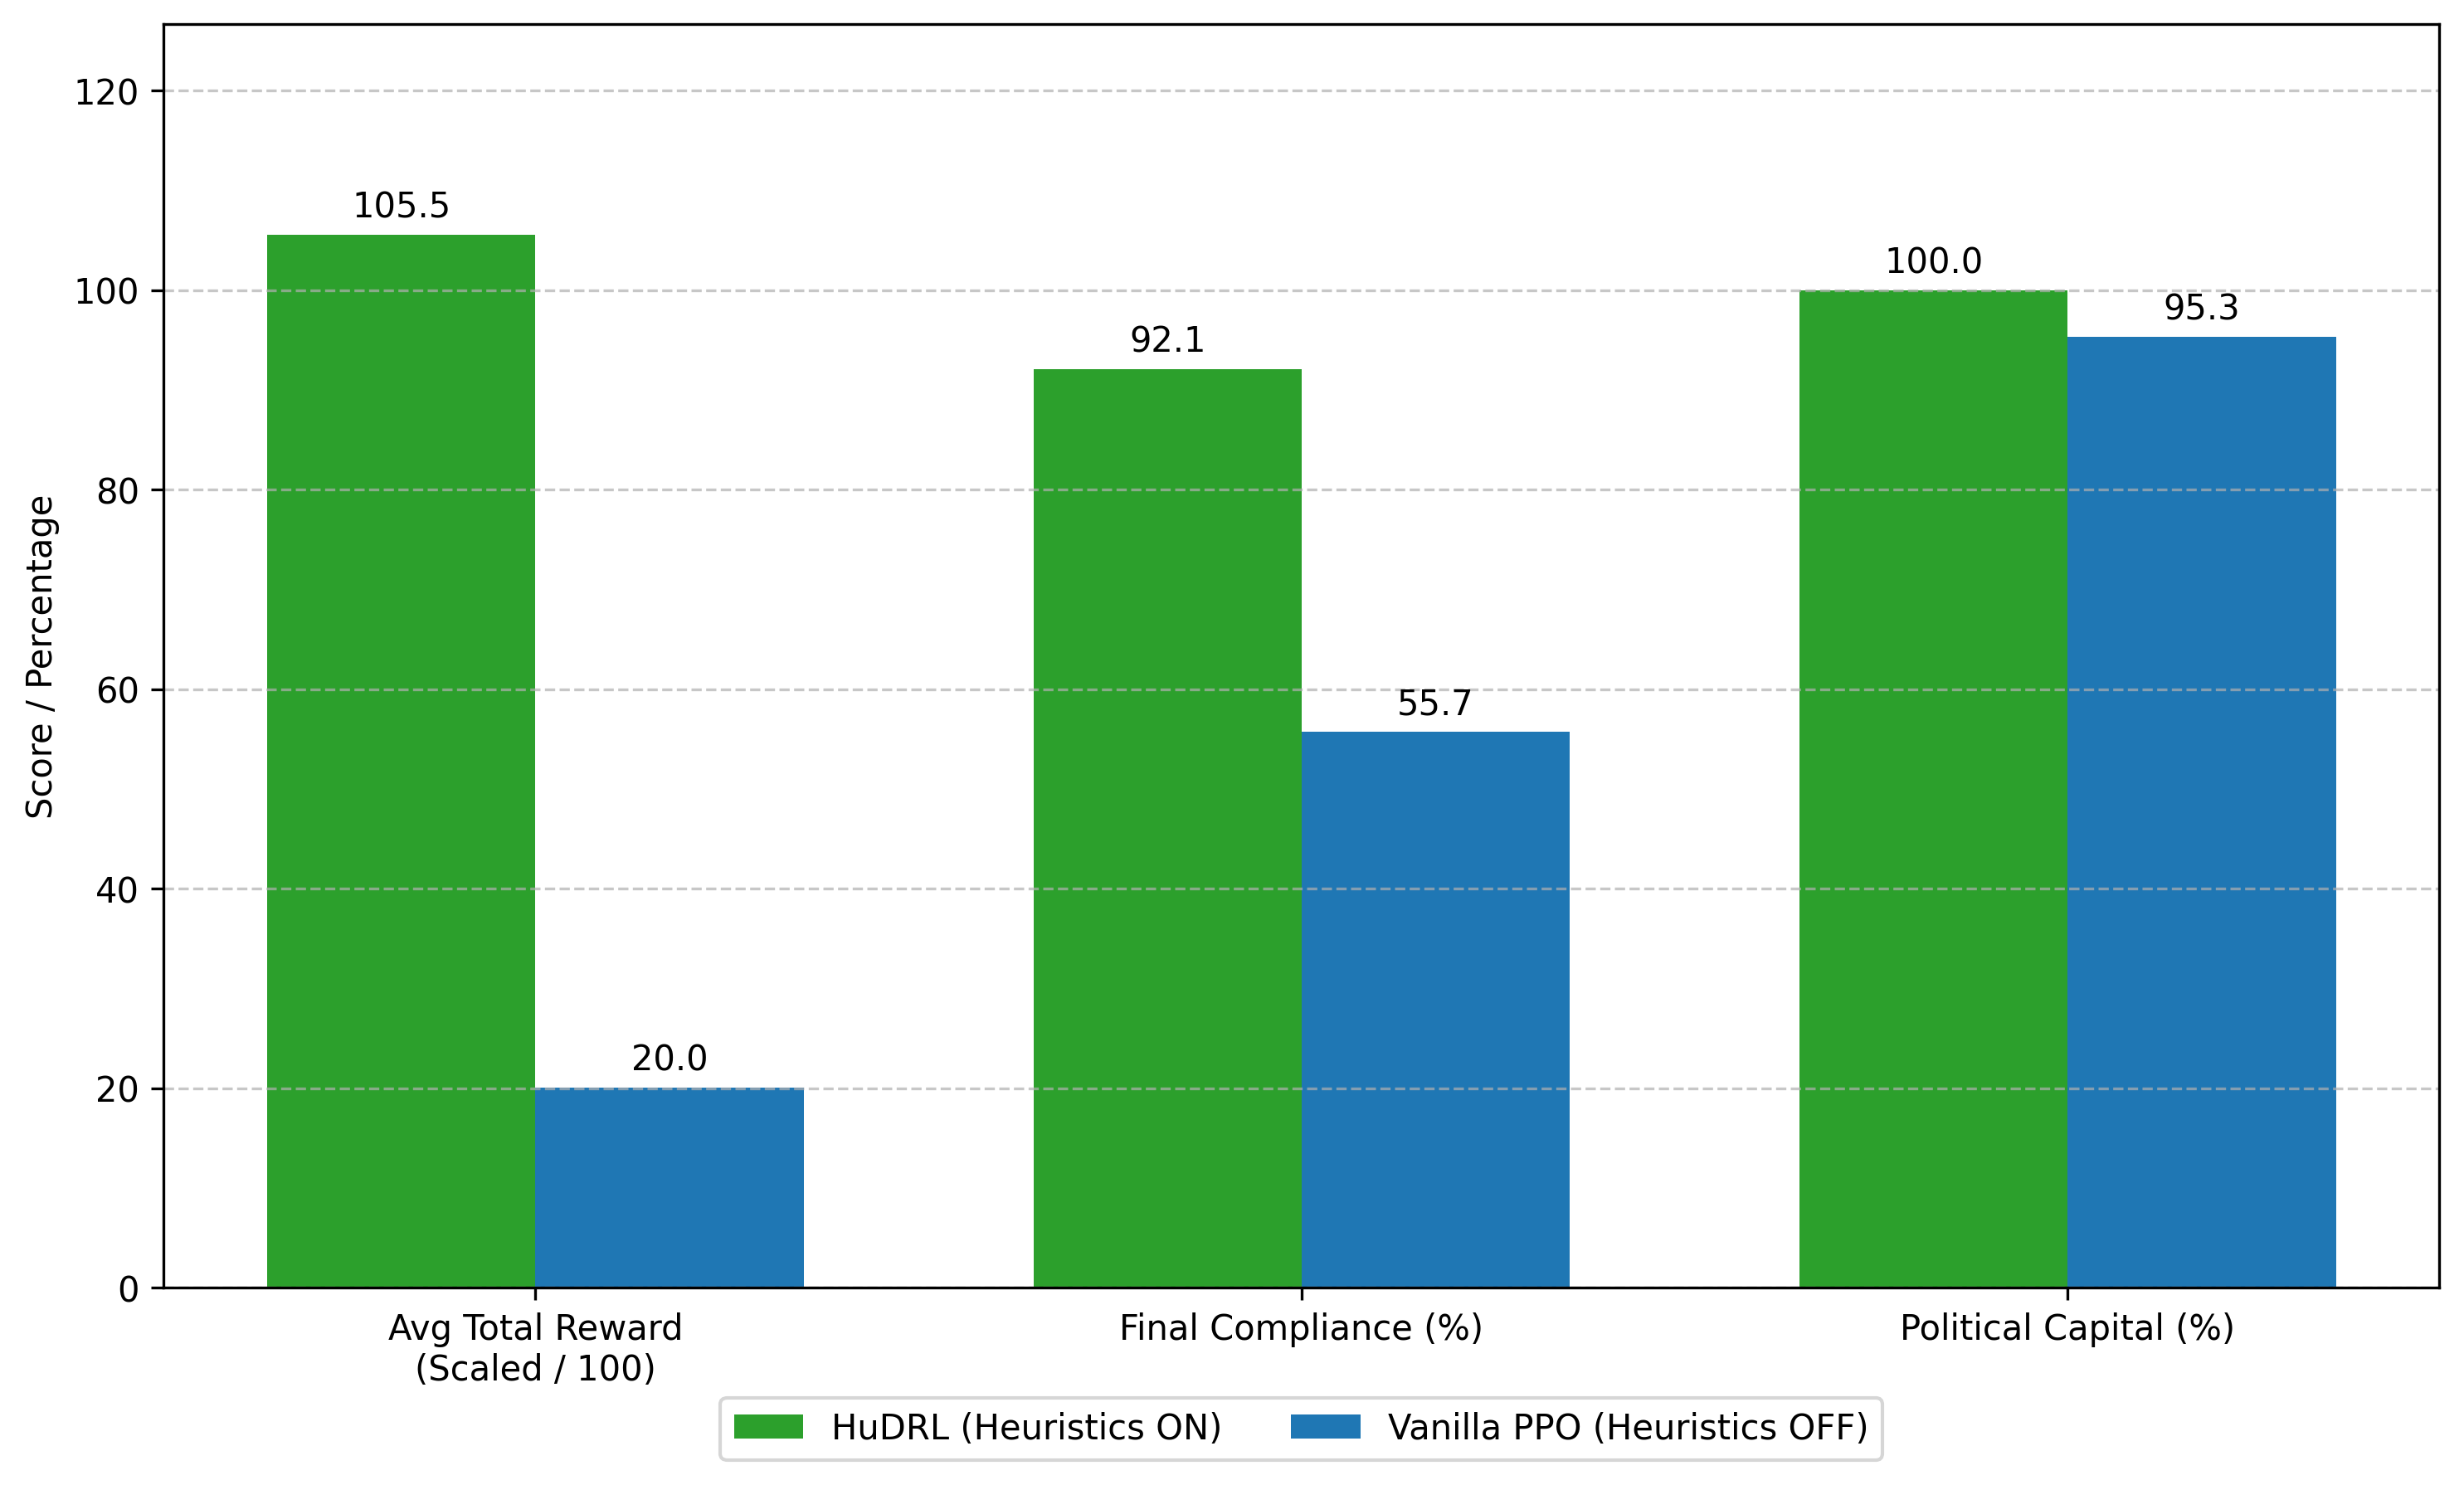
\includegraphics[width=0.85\columnwidth]{images/hudrl_vs_vanilla.png}
    \caption{Performance Comparison of HuDRL vs. Baseline PPO}
    \label{fig:heuristic_vs_non_heuristic}
    \vspace{-0.3cm}
\end{figure}

\subsection{Comparative Analysis of Policy Strategies}
Simulation experiments over a three-year horizon demonstrated a stark divergence between traditional heuristics and DRL optimization. The ``Status Quo'' baseline policy, which distributed the municipal budget equally across the barangays, acted as a dilution mechanism. Funds were spread too thin to cross the behavioral tipping point, resulting in a terminal global compliance of only 30.18\%. The contrast in compliance rate trajectories is depicted in Figure \ref{fig:comparison_policy_graph}.

\begin{figure}[H] 
\centering
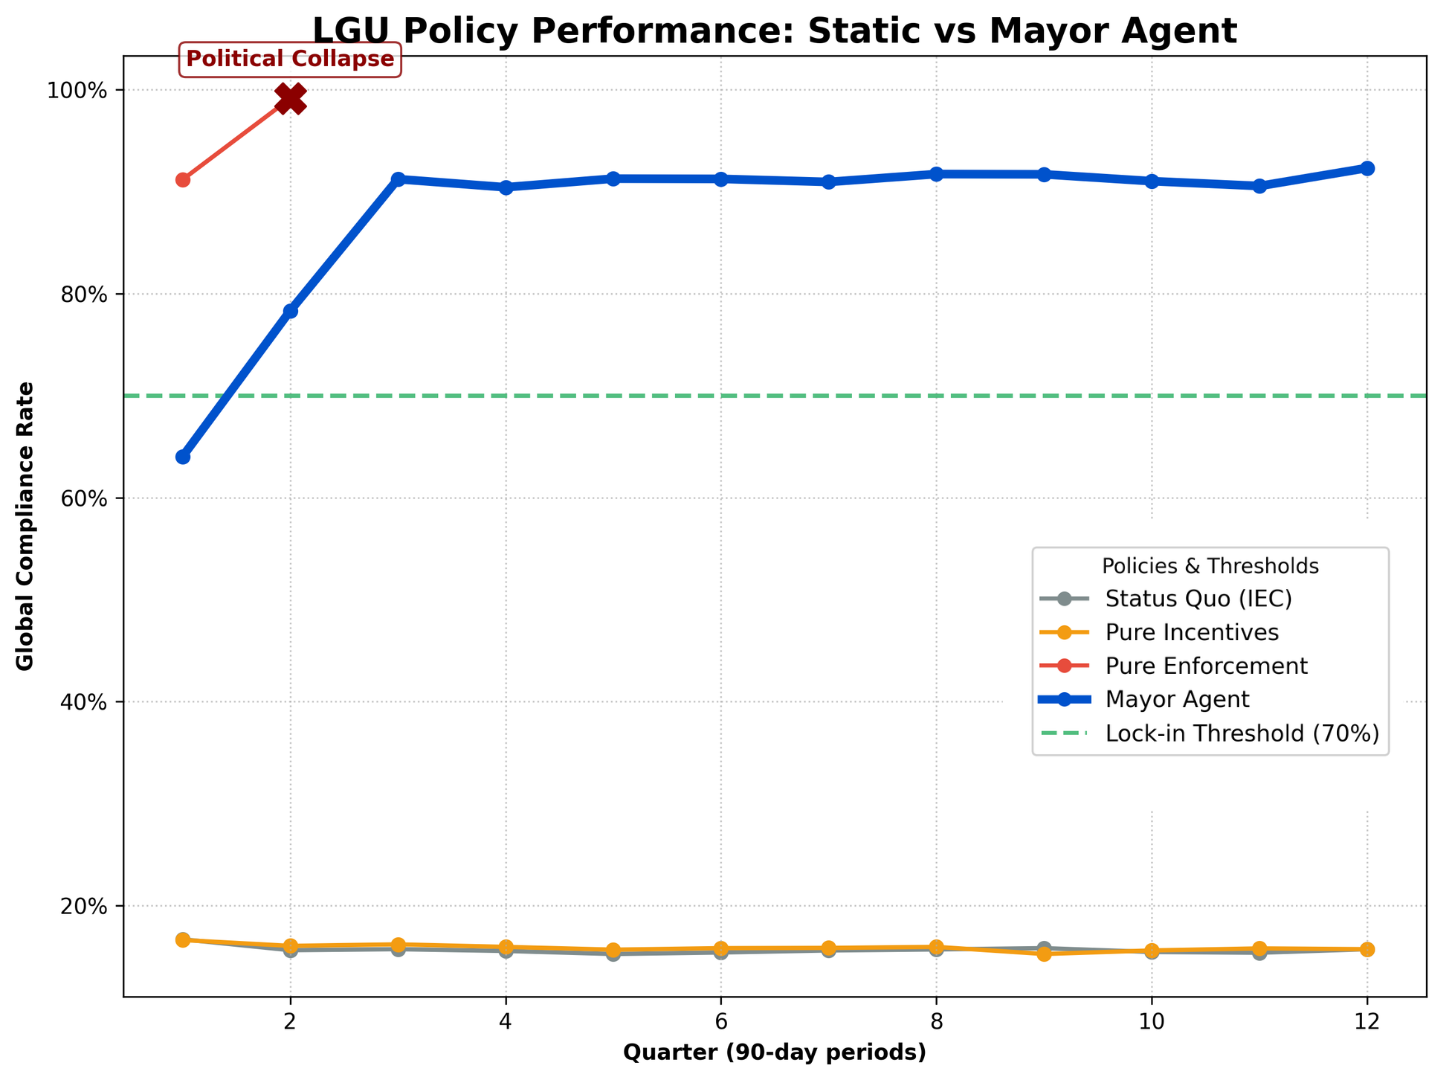
\includegraphics[width=0.85\columnwidth]{images/comparison_policy_strategy.png}
\caption{Compliance Rate Performances of Simulated Policy Strategies}
\label{fig:comparison_policy_graph}
\vspace{-0.3cm}
\end{figure}

In contrast, the HuDRL Mayor Agent autonomously discovered an aggressive ``Sequential Saturation'' strategy, achieving 90.45\% global compliance. By bypassing human intuitive biases toward ``fair'' simultaneous distribution, the AI concentrated up to 69\% of its budget onto single barangays sequentially. After pushing a locale past the 70\% norm internalization threshold, the AI effectively triggered the Graduation Effect \cite{centola2018}. It then ceased funding that stabilized area—relying entirely on cultural inertia to prevent behavioral decay—and pivoted its fiscal arsenal to besiege the next municipal bottleneck.

\section{Conclusion}
This study proves that coupling Agent-Based Modeling with Heuristic-Guided DRL provides a powerful, risk-free virtual laboratory for optimizing complex public policy. By formulating the Municipality of Bacolod as an MDP, the AI demonstrated that overcoming logistical friction through targeted, sequential saturation of resources is mathematically superior to broad, diluted educational mandates. However, a primary limitation of the current framework is that the meso-level barangay nodes operate predominantly as passive policy receivers rather than fully adaptive, independent strategists. Future work will explore expanding this architecture into Multi-Agent Reinforcement Learning (MARL), empowering barangays to operate as autonomous sub-agents that dynamically negotiate for municipal funding \cite{zheng2022b}.

\section*{Acknowledgment}
The authors thank the Bacolod LGU for providing essential audit data and the MSU-IIT Department of Computer Science for their continued support.

\section*{Usage of Generative AI}
Generative AI was used solely for language editing and formatting; all core research, data analysis, and algorithmic design are the authors' original work.

\section*{Conflict of Interest}
The authors declare no conflicts of interest.

\begin{thebibliography}{00}

\bibitem{ra9003} Republic of the Philippines, ``Ecological Solid Waste Management Act of 2000, Rep. Act No. 9003,'' Jan. 2001.

\bibitem{tian2024} X. Tian, et al., ``Agent-based modeling in solid waste management: Advantages, progress, challenges and prospects,'' \textit{Env. Impact Assess. Rev.}, vol. 110, p. 107723, 2024.

\bibitem{centola2018} D. Centola, J. Becker, D. Brackbill, and A. Baronchelli, ``Experimental evidence for tipping points in social convention,'' \textit{Science}, vol. 360, no. 6393, pp. 1116--1119, 2018.

\bibitem{andre2021} P. Andre, T. Boneva, F. Chopra, and A. Falk, ``Fighting climate change: The role of norms, preferences, and moral values,'' \textit{Working Paper}, 2021.

\bibitem{paigalan2025} S. J. L. Paigalan, et al., ``Knowledge, attitude, and practices on solid waste management among residents of a riverside barangay,'' \textit{Scientia}, vol. 2, no. 5, pp. 3--14, 2025.

\bibitem{zhao2022} A. Zhao, L. Zhang, X. Ma, F. Gao, and H. Zhu, ``Effectiveness of extrinsic incentives for promoting rural waste sorting in developing countries,'' \textit{The Developing Economies}, vol. 60, no. 3, 2022.

\bibitem{taraghi2025} M. Taraghi and L. Yoder, ``Integrating the theory of planned behavior in agent-based models: A systematic review,'' \textit{Ecological Modelling}, vol. 508, p. 111231, 2025.

\bibitem{zheng2022b} S. Zheng, et al., ``The AI Economist: Taxation policy design via two-level deep multiagent reinforcement learning,'' \textit{Science Advances}, vol. 8, no. 18, 2022.

\bibitem{sobol2001} I. M. Sobol, ``Global sensitivity indices for nonlinear mathematical models and their monte carlo estimates,'' \textit{Math. and Computers in Simulation}, vol. 55, no. 1-3, pp. 271-280, 2001.

\bibitem{nishimura2022} K. Nishimura, ``How does decentralization affect the performance of municipalities in urban environmental management in the Philippines?,'' \textit{Lex Localis Journal of Local Self-Government}, vol. 20, no. 4, pp. 715-738, 2022.

\bibitem{yazawa2025} T. Yazawa, et al., ``Act and reality of the ecological solid waste management act on barangay-level waste management in Barbaza, the Philippines,'' \textit{Discover Sustainability}, vol. 6, no. 1, 2025.

\bibitem{moeini2023} B. Moeini, et al., ``Effect of household interventions on promoting waste segregation behavior at source: A systematic review,'' \textit{Sustainability}, vol. 15, no. 24, p. 16546, 2023.

\bibitem{udayakumar2023} R. Udayakumar, et al., ``Improved particle swarm optimization with deep learning-based municipal solid waste management in smart cities,'' \textit{Revista de Gestão Social e Ambiental}, vol. 17, no. 4, p. e03561, 2023.

\end{thebibliography}

\end{document}